\documentclass[10pt]{standalone}
\usepackage{amsmath}
\usepackage{pgf,tikz}
\usepackage{mathrsfs}
\usetikzlibrary{arrows}
\pagestyle{empty}
\begin{document}

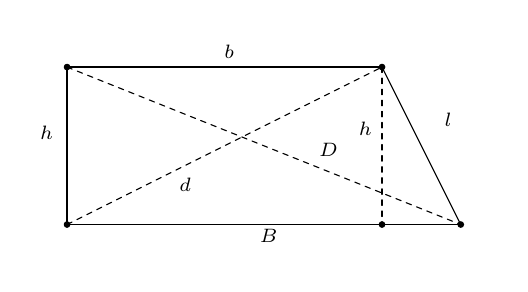
\begin{tikzpicture}[line cap=round,line join=round,>=triangle 45,x=1.0cm,y=1.0cm]



\clip(-2.5,-0.5) rectangle (3.5,2.5);
\draw  (-2.,0.)-- (3.,0.);
\draw  (3.,0.)-- (2.,2.);
\draw  (2.,2.)-- (-2.,2.);
\draw  (-2.,2.)-- (-2.,0.);
\draw [dash pattern=on 2pt off 2pt] (-2.,2.)-- (3.,0.);
\draw [dash pattern=on 2pt off 2pt] (-2.,0.)-- (2.,2.);
\draw [dash pattern=on 2pt off 2pt] (2.,2.)-- (2.,0.);
\begin{scriptsize}
\draw [fill=black] (-2.,0.) circle (1.0pt);
\draw [fill=black] (3.,0.) circle (1.0pt);

\draw [fill=black] (2.,2.) circle (1.0pt);

\draw [fill=black] (-2.,2.) circle (1.0pt);
\draw [fill=black] (2.,0.) circle (1.0pt);

\draw[color=black] (2.84,1.33) node {$l$};
\draw[color=black] (0.06,2.2) node {$b$};
\draw[color=black] (-2.26,1.17) node {$h$};
\draw[color=black] (1.32,0.95) node {$D$};
\draw[color=black] (-0.5,0.5) node {$d$};
\draw[color=black] (1.79,1.22) node {$h$};
\draw[color=black] (0.56,-0.15) node {$B$};
\end{scriptsize}
\end{tikzpicture}
\end{document}